\documentclass[%
12pt, %
final, % 
oneside, % 
onecolumn, %  
centertags]{article} % относится к классу article и размер шрифта 12 пунктовб, {article: статья, report: отчеты и диссертации, book: книга, letter: письмо}

% \usepackage{fontspec}
 
% \setmainfont{Times New Roman}

% \documentclass[a4paper, 12pt]{report}

\topmargin= -30pt % насколько сверху будет страница
\textheight= 650pt


\usepackage[utf8]{inputenc} % задает кодировку, utf-8 кодировка, включающая в себя знаки почти всех языков мира
\usepackage[english]{babel} % подключает необходимые языки, основным языком является английский

\selectlanguage{english} % настройки будут на английском, но писать будет на русском

\usepackage{euscript}
\usepackage{supertabular}

\renewcommand{\baselinestretch}{1.0} 

\usepackage[colorlinks=true,linkcolor=blue,unicode=true,urlcolor = blue]{hyperref} %hypered
\usepackage[pdftex]{graphicx} % для графики

\usepackage{amsthm, amssymb, amsmath, amsfonts} % математический пакет, математические шрифты
\usepackage{textcomp}
\usepackage[noend]{algorithmic}
\usepackage[ruled]{algorithm}
\usepackage{lipsum}
\usepackage{indentfirst}
\usepackage{babel}
\usepackage{pgfplots}
\usepackage{setspace}
\usepackage{xcolor}
\usepackage{hyperref}
\usepackage{subfigure}

\setcounter{secnumdepth}{5}
\setcounter{tocdepth}{5}
\newcommand\simpleparagraph[1]{%
  \stepcounter{paragraph}\paragraph*{\theparagraph\quad{}#1}}
\usepackage{listings}
% \usepackage{xcolor}
%\usepackage{minted}

\lstset { %
     language=C++,
     backgroundcolor=\color{black!5}, % set backgroundcolor
     basicstyle=\footnotesize,% basic font setting
}


\linespread{1.0} 
\setlength{\parindent}{2.4em}
\setlength{\parskip}{0.1em}

\pgfplotsset{compat=1.9}
\pgfplotsset{model/.style = {blue, samples = 100}} 
\pgfplotsset{experiment/.style = {red}}

\theoremstyle{plain}
\binoppenalty=10000

\newtheorem{theorem}{Theorem}[section] % theorem

\theoremstyle{definition}
% \newtheorem{definition}{Определение}[subsection]
\newtheorem{definition}{Definition}[subsection]

\theoremstyle{remark}
% \newtheorem{remark}{Замечание}[section]

% \newtheorem{corollary}{Следствие}

% \newtheorem{proposition}{Proposition}

% \newtheorem{example}{Пример}

% \newtheorem{lemma}{Лемма}[section]

\renewcommand*{\proofname}{Proof}

\graphicspath{ {./images/} }


% \usepackage{amsmath,amsfonts,amssymb, setspace}  % Разнообразные математические команды и значки
% \usepackage{indentfirst}     % Отступ в первом абзаце

% \pagestyle{empty}
\usepackage[left=2.5cm, right=1.5cm, top=2.5cm, bottom=2.5cm]{geometry}
\usepackage[medium]{titlesec}
\usepackage{graphicx}
% \graphicspath{ {./images/} }

\begin{document}

	\begin{titlepage} 
		\begin{center}
		\textbf{}\\[2.0cm]
		\LARGE FEDERAL STATE AUTONOMOUS EDUCATIONAL INSTITUTION OF HIGHER EDUCATION \\[0.5cm]
		\Large ITMO UNIVERSITY \\[3cm]
		\LARGE Report\\
		\Large OpenMP. Practical tasks No. $1-3$. \\
		\Large Parallel algorithms for the analysis and synthesis of data \\[4cm]


		\begin{flushright}
		Performed by\\
		Aleksandr Shirokov\\
		J4133c\\
		Accepted by\\
		Petr Andriushchenko
		\end{flushright}

		\vfill 

		{\Large {St. Petersburg}} \par
		{\Large {2021}}
		\end{center} 
	\end{titlepage}

\tableofcontents
\newpage

\section{Assignments}

\subsection{Assignment 0.}

\subsubsection{Formulation of the problem}

Write a program for counting words in a line. Any sequence of characters without 
separators is considered a word. Separators are spaces, tabs, newlines.

The input string is passed to the program through the terminal as the $\operatorname{argv} [1]$ 
parameter. The program should display the number of words on the screen.

\subsubsection{Detailed description of solution}

Description of algorithm: until the line ends, check for the new words and check for separators which are not new words.

\subsubsection{Example of launch parameters and output}

Code for \textbf{assignment 0} is \href{https:\//github.com/aptmess/parallel_algorithms/blob/master/HT/hw_openmp/prog/A0.cpp}{here}.

Compilation example: 

\begin{itemize}
	\item \textsc{g++ -o ./cpf/A0.o A0.cpp}
	\item The same instruction wrote in sh file: \textsc{sh build\_task1.sh}
\end{itemize}

Launch example: \textsc{./cpf/A0.o 'my string'}

\begin{center}
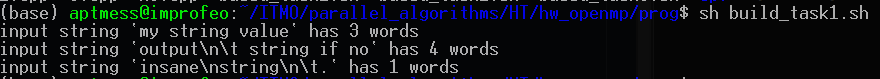
\includegraphics[scale=0.8]{t1.png}

Pic. 1. Output results for assignment 0
\end{center}

Here are some examples that shows that algorithm works correctly - it skips separators and return correct amount of words.

\newpage

\subsection{Assignment 1. Finding the maximum value of a vector}

\subsubsection{Formulation of the problem}

\begin{enumerate}
	\item Write a parallel \textsc{OpenMP} program that finds the maximum value of a vector (one-dimensional array). Each thread should only store its maximum value; concurrent access to a shared variable that stores the maximum value is not allowed.
	\item Study the dependence of the runtime on the number of threads used (from $1$ to $10$) for a vector that contains at least $1,000,000$ elements (the more, the better).
	\item Check the correctness of the program on $10$ elements.
	\item The program should display on the screen: the number of threads, the execution 
time.
	\item Transfer the size of the vector through the $\operatorname{argv} [1]$ parameter.
\end{enumerate}

\subsubsection{Detailed description of solution}

\begin{itemize}
	\item Wrote two functions
	\begin{enumerate}
		\item \textsc{max}.
		\begin{enumerate}
			\item Input parameters: array (\textsc{arr}), len of array (\textsc{len}), amount of threads (\textsc{threads})
			\item Detailed description: takes the first element of array as a \textsc{maximum}, use \textsc{\#pragma omp parallel for num\_threads(threads) reduction(max:maximum)} - using parallel loop for with reduction to find maximum element. Inside loop - compare elements with each maximum in thread. Reference to \href{https:\//stackoverflow.com/questions/35629261/max-value-in-an-array-using-openmp}{this one}.
			\item Output parameters: maximum
		\end{enumerate}
		\item \textsc{generate\_array}: returns random int array of size \textsc{len} in range $[1, \operatorname{len} + \operatorname{int}(0.4 \cdot \operatorname{len})]$
	\end{enumerate}
	\item Calculated for each amount of thread time using function \textsc{omp\_get\_wtime()}
	\item Used \textsc{srand(time(NULL))} to make different generation of array for each run
	\item Used \textsc{atoi} function to convert the argv value to an int with \textsc{<cstdlib>} library
\end{itemize}

\subsubsection{Example of launch parameters and output}

Code for \textbf{assignment 1} is \href{https:\//github.com/aptmess/parallel_algorithms/blob/master/HT/hw_openmp/prog/2.cpp}{here}.

Compilation example: 

\begin{itemize}
	\item \textsc{g++ -o ./cpf/2.o 2.cpp -fopenmp}
	\item The same instruction wrote in sh file: \textsc{sh build\_task2.sh 100} (the second parameter is the length of array)
\end{itemize}

Launch example: \textsc{./cpf/2.o 100}

Let's analyse the results. Firstly, let's prove, that algorithm works correctly.
\begin{center}

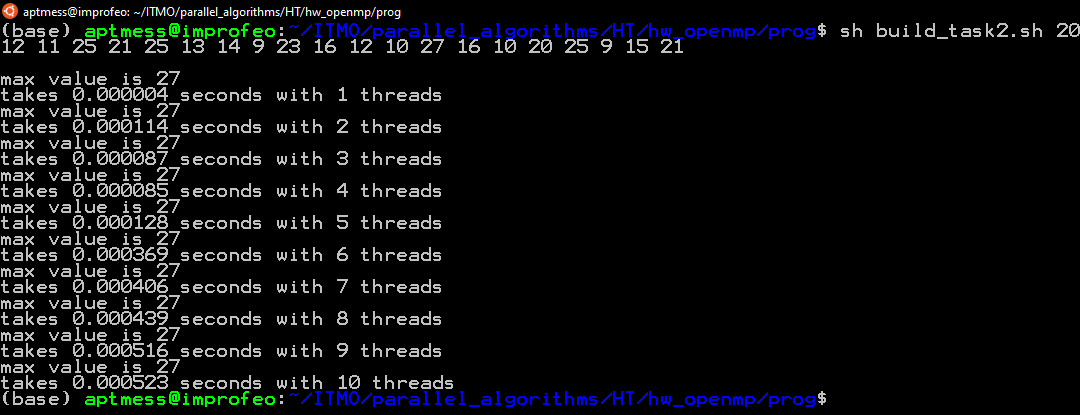
\includegraphics[scale=0.61]{t2_check.png}

Pic. 2. Input size of array - 20
\end{center}

As we can see, the worker with only $1$ thread on lower sizes of array's work quicklier than with the bigger amount of threads cause for threads the program needs time to create them as we discuseed on lecture. This behaviour ot the program works till $10000$, but let's check the time on bigger input size of arrays.

\begin{center}
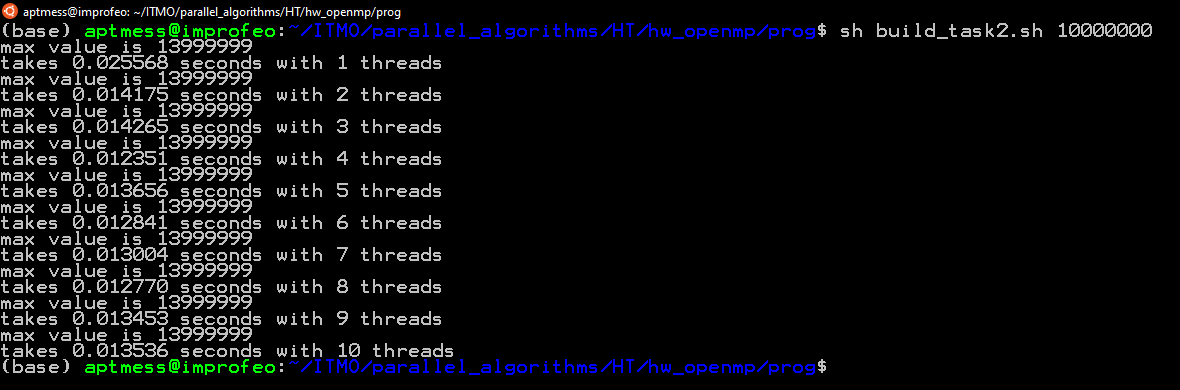
\includegraphics[scale=0.55]{t2_10_billions.png}

Pic. 3. Input size of array - 10 millions
\end{center}

\begin{center}
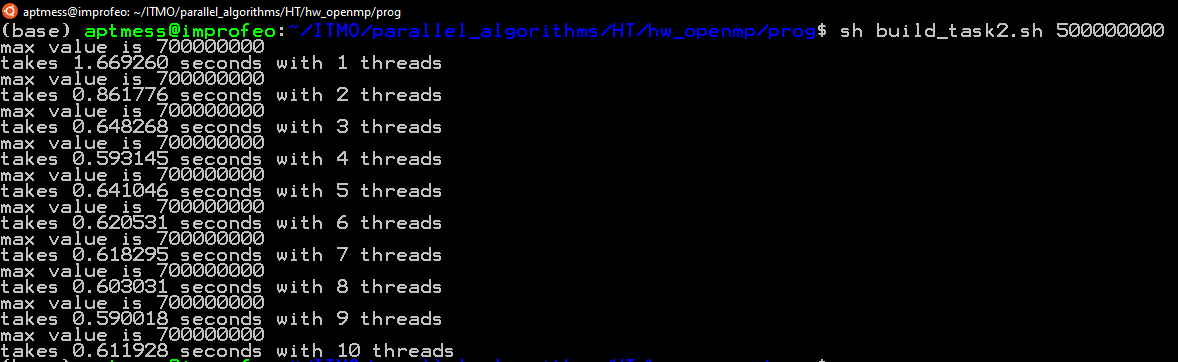
\includegraphics[scale=0.55]{t2_500_mil.png}

Pic. 4. Input size of array - 500 millions
\end{center}

\begin{center}
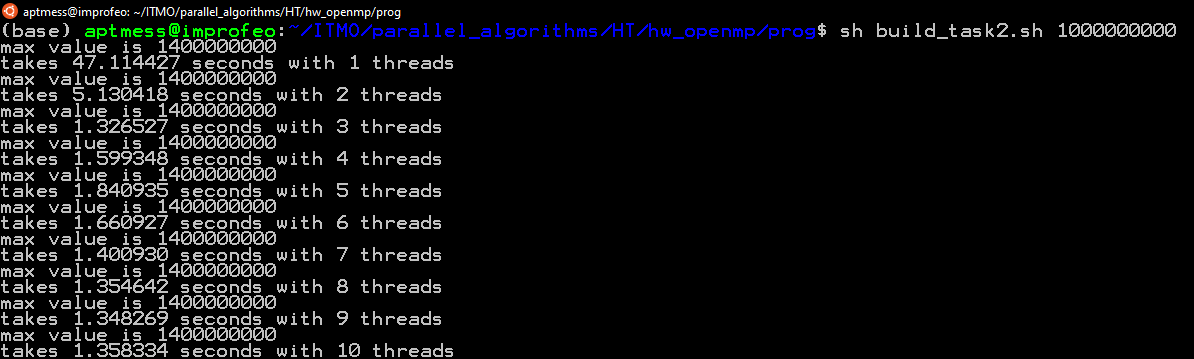
\includegraphics[scale=0.55]{t2_billion.png}

Pic. 5. Input size of array - 1 billion
\end{center}

Let's visualise the last table of results on a scatter plot.


\begin{center}
	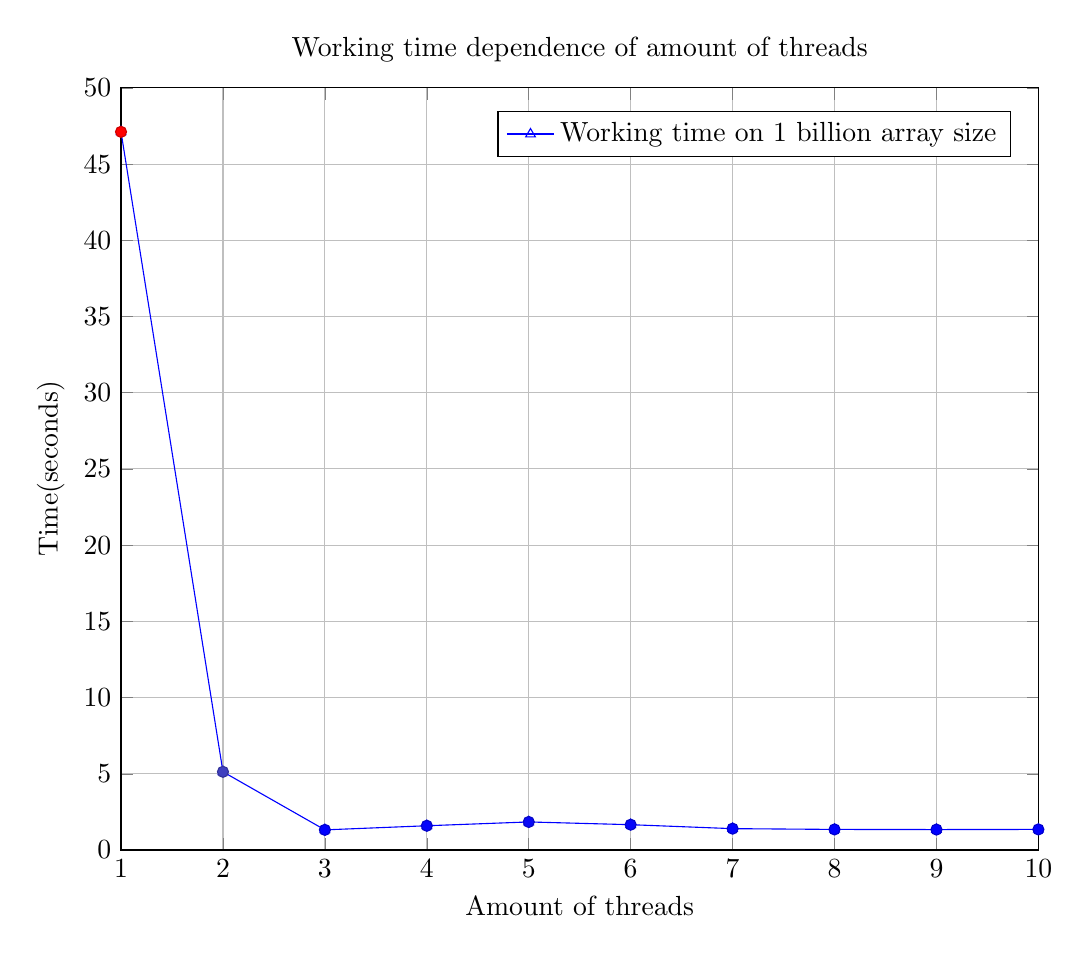
\begin{tikzpicture}
		\begin{axis}[
		xmin = 1, 
		xmax = 10,
		ymin = 0, 
		ymax = 50, 
		grid = major,
		scale = 1.7,
		legend pos = north east,
		title={Working time dependence of amount of threads},
		xlabel={Amount of threads},
		ylabel={Time(seconds)},
		]
		\legend{Working time on 1 billion array size};
	\addplot[color=blue, mark=triangle] coordinates { (1, 47.114427) (2,5.13) (3,1.32) (4,1.59) (5,1.84) (6,1.66) (7,1.4) (8,1.35) (9,1.34) (10,1.35)} ;
	\addplot[scatter,only marks] coordinates { (1, 47.114427) (2,5.13) (3,1.32) (4,1.59) (5,1.84) (6,1.66) (7,1.4) (8,1.35) (9,1.34) (10,1.35)} ;
		\end{axis}
	\end{tikzpicture}
\end{center}

So, we can make some thoughts from the results - firsly with increasing amount of input array size the working time of program with $1$ thread is the slowest between programs with other amount of threads, also program with $2$ threads is slower than others. Since program has $3$ thread the working time of algorithms are more or less the same, but we can clearify that with the bigger amount of thread the working time of program is less and in common from $1$ thread to $10$ working time decreases more or less exponential. Mention one more time, that on lower size of arrays the working time of algorithm with $1$ thread is the quickiest.

Let's move to the third assignment.

\newpage

\subsection{Assignment 2. Matrix multiplication}

\subsubsection{Formulation of the problem}

\begin{enumerate}
	\item Write a program for multiplying two square matrices using \textsc{OpenMP}. 
	\item Examine the performance of different modifications of the algorithm (different loop order), depending on the number of threads used for matrices of at least $800 \times 800$.
	\item Check the correctness of the multiplication on $5 \times 5$ matrices.
	\item Calculate the efficiency by the formula $\frac{t_1}{t}$ where:
	\begin{itemize}
		\item $t_1$ - multiplication time on only one thread
		\item $t$ - multiplication time on $n$ threads (the number of streams is taken from $1$ to $10$).
	\end{itemize}
	\item The program should output number of threads, multiplication time and efficiency.
	\item Transfer the size of matrices through the $\operatorname{argv} [1]$ parameter.
\end{enumerate}

\subsubsection{Detailed description of solution}

I have used an implemetation of lecture's file \textsc{matrix\_multiplication.cpp} and add some feature to parallelize it and make output result. Other thins are absolutely the same. Mention the main points of program:

\begin{itemize}
	\item Used functions to allocate memory for two dimensional array (\textsc{malloc\_array}), initializing a matrix with random integer from $1$ to $10$
	\item Used \textsc{\#pragma omp parallel for num\_threads(threads)} for paralleling operations
	\item For each thread and for each permutation ($4$ permutations: ijk, ikj, jik, jki) calculate working time and put the results in matrix $4 \times 10$, where $4$ is amount of permutation and $10$ - the amount of threads
	\item This table has pretty nice visualisation
	\item Calculated for each amount of thread time using function \textsc{omp\_get\_wtime()}
	\item Used \textsc{srand(time(NULL))} to make different generation of array for each run
	\item Used \textsc{atoi} function to convert the argv value to an int with \textsc{<cstdlib>} library
	\item Compare results with matrix multiplication without parallel
\end{itemize}

\subsubsection{Example of launch parameters and output}

Code for \textbf{assignment 2} is \href{https:\//github.com/aptmess/parallel_algorithms/blob/master/HT/hw_openmp/prog/3.cpp}{here}.

Compilation example: 

\begin{itemize}
	\item \textsc{g++ -o ./cpf/3.o 3.cpp -fopenmp}
	\item The same instruction wrote in sh file: \textsc{sh build\_task3.sh 1000} (the second parameter is the size of matrices)
\end{itemize}

Launch example: \textsc{./cpf/3.o 5}

Let's analyse the results. Firstly, let's prove, that algorithm works correctly.

\begin{figure}[h!]
    \centering
    \subfigure{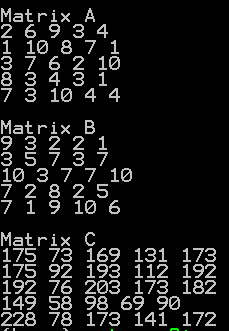
\includegraphics[width=0.24\textwidth]{res_3.png}} 
    \subfigure{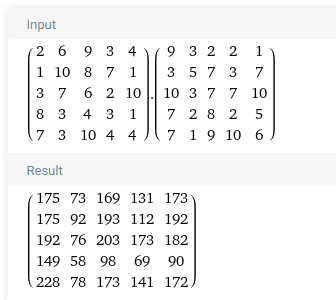
\includegraphics[width=0.4\textwidth]{wf_3.png}} 

    Pic. 6. The results of program work and wolfram alpha are the same!
\end{figure}

Launch our program with matrix size $1000 \times 1000$ and wait for the results. (1 year later) let' see them!

\begin{center}
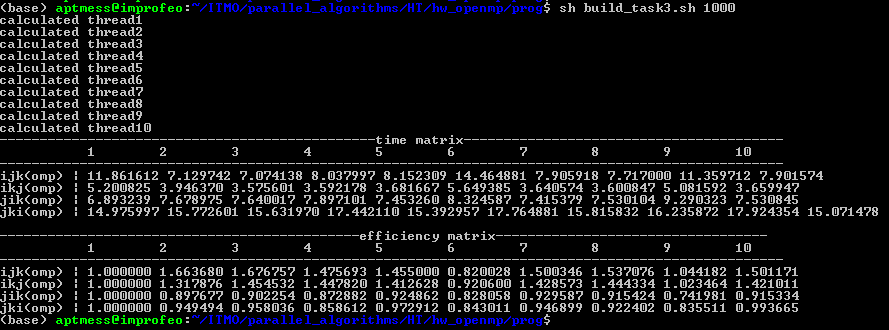
\includegraphics[scale=0.65]{df_3.png}

Pic. 7. Time Matrix, Efficeincy matrix and working time without parallel (thread 1)
\end{center}

As we can see the increasing amount of threads doesn't always decrease the working time, as we can see in permutation jik and jki, but in ikj the time decreases with the increasing amount of threads and due to time comparison it is the best way fro matrix mupltiplication. But we have to mention, that our program with many threads works quicklier than the program with $1$ thread, so parallezation helps.

Analzying of algorithm can improve working time of algorithms in many times, so we should be careful when we choose algorithm.

\subsection{Appendix}

The link to the sourse code which is placed on my \href{https://github.com/aptmess/parallel_algorithms}{github}.


\end{document}